\section{Description of OpenVAS Setup} \label{sec:setup}

\inlinetodo{
This section should include a brief explanation of how the architecture of OpenVAS and a description of the setup of the scanned network. Try to find some references about OpenVAS and vulnerability scanning in general and write briefly:
 \newline
~\ \newline 
  \textbullet\ Why scanning is a useful method? What are the types of vulnarability scanning?
\newline
  \textbullet\ What do we expect from the scanning results? 
\newline
  \textbullet\ How to perform it by OpenVAS? 
\newline
~\ \newline 
\textbf{Note: }Do not forget to add references at the end of the report and refer to them in the text here. 
\newline
~\ \newline 
This section should also describe the scans you are considering, including the chosen NVT families used (and possible exception or specific NVTs chosen) with their settings and parameters (in each step below). Explain in each step:
\newline
~\ \newline 
  \textbullet\ Why you choose the different NVTs and the chosen configurations?
\newline
  \textbullet\ What are the aim of the different scans and why did you make the different choices? For example, why did you only scan specific ports in your port scanning. Give details and motivations. 
 \newline
~\ \newline
References to figure should be included in the text, e.g., ''In Figure~\ref{fig:setup}, 
the network setup is described\ldots'' }

\begin{figure}[htb]
  \centering
  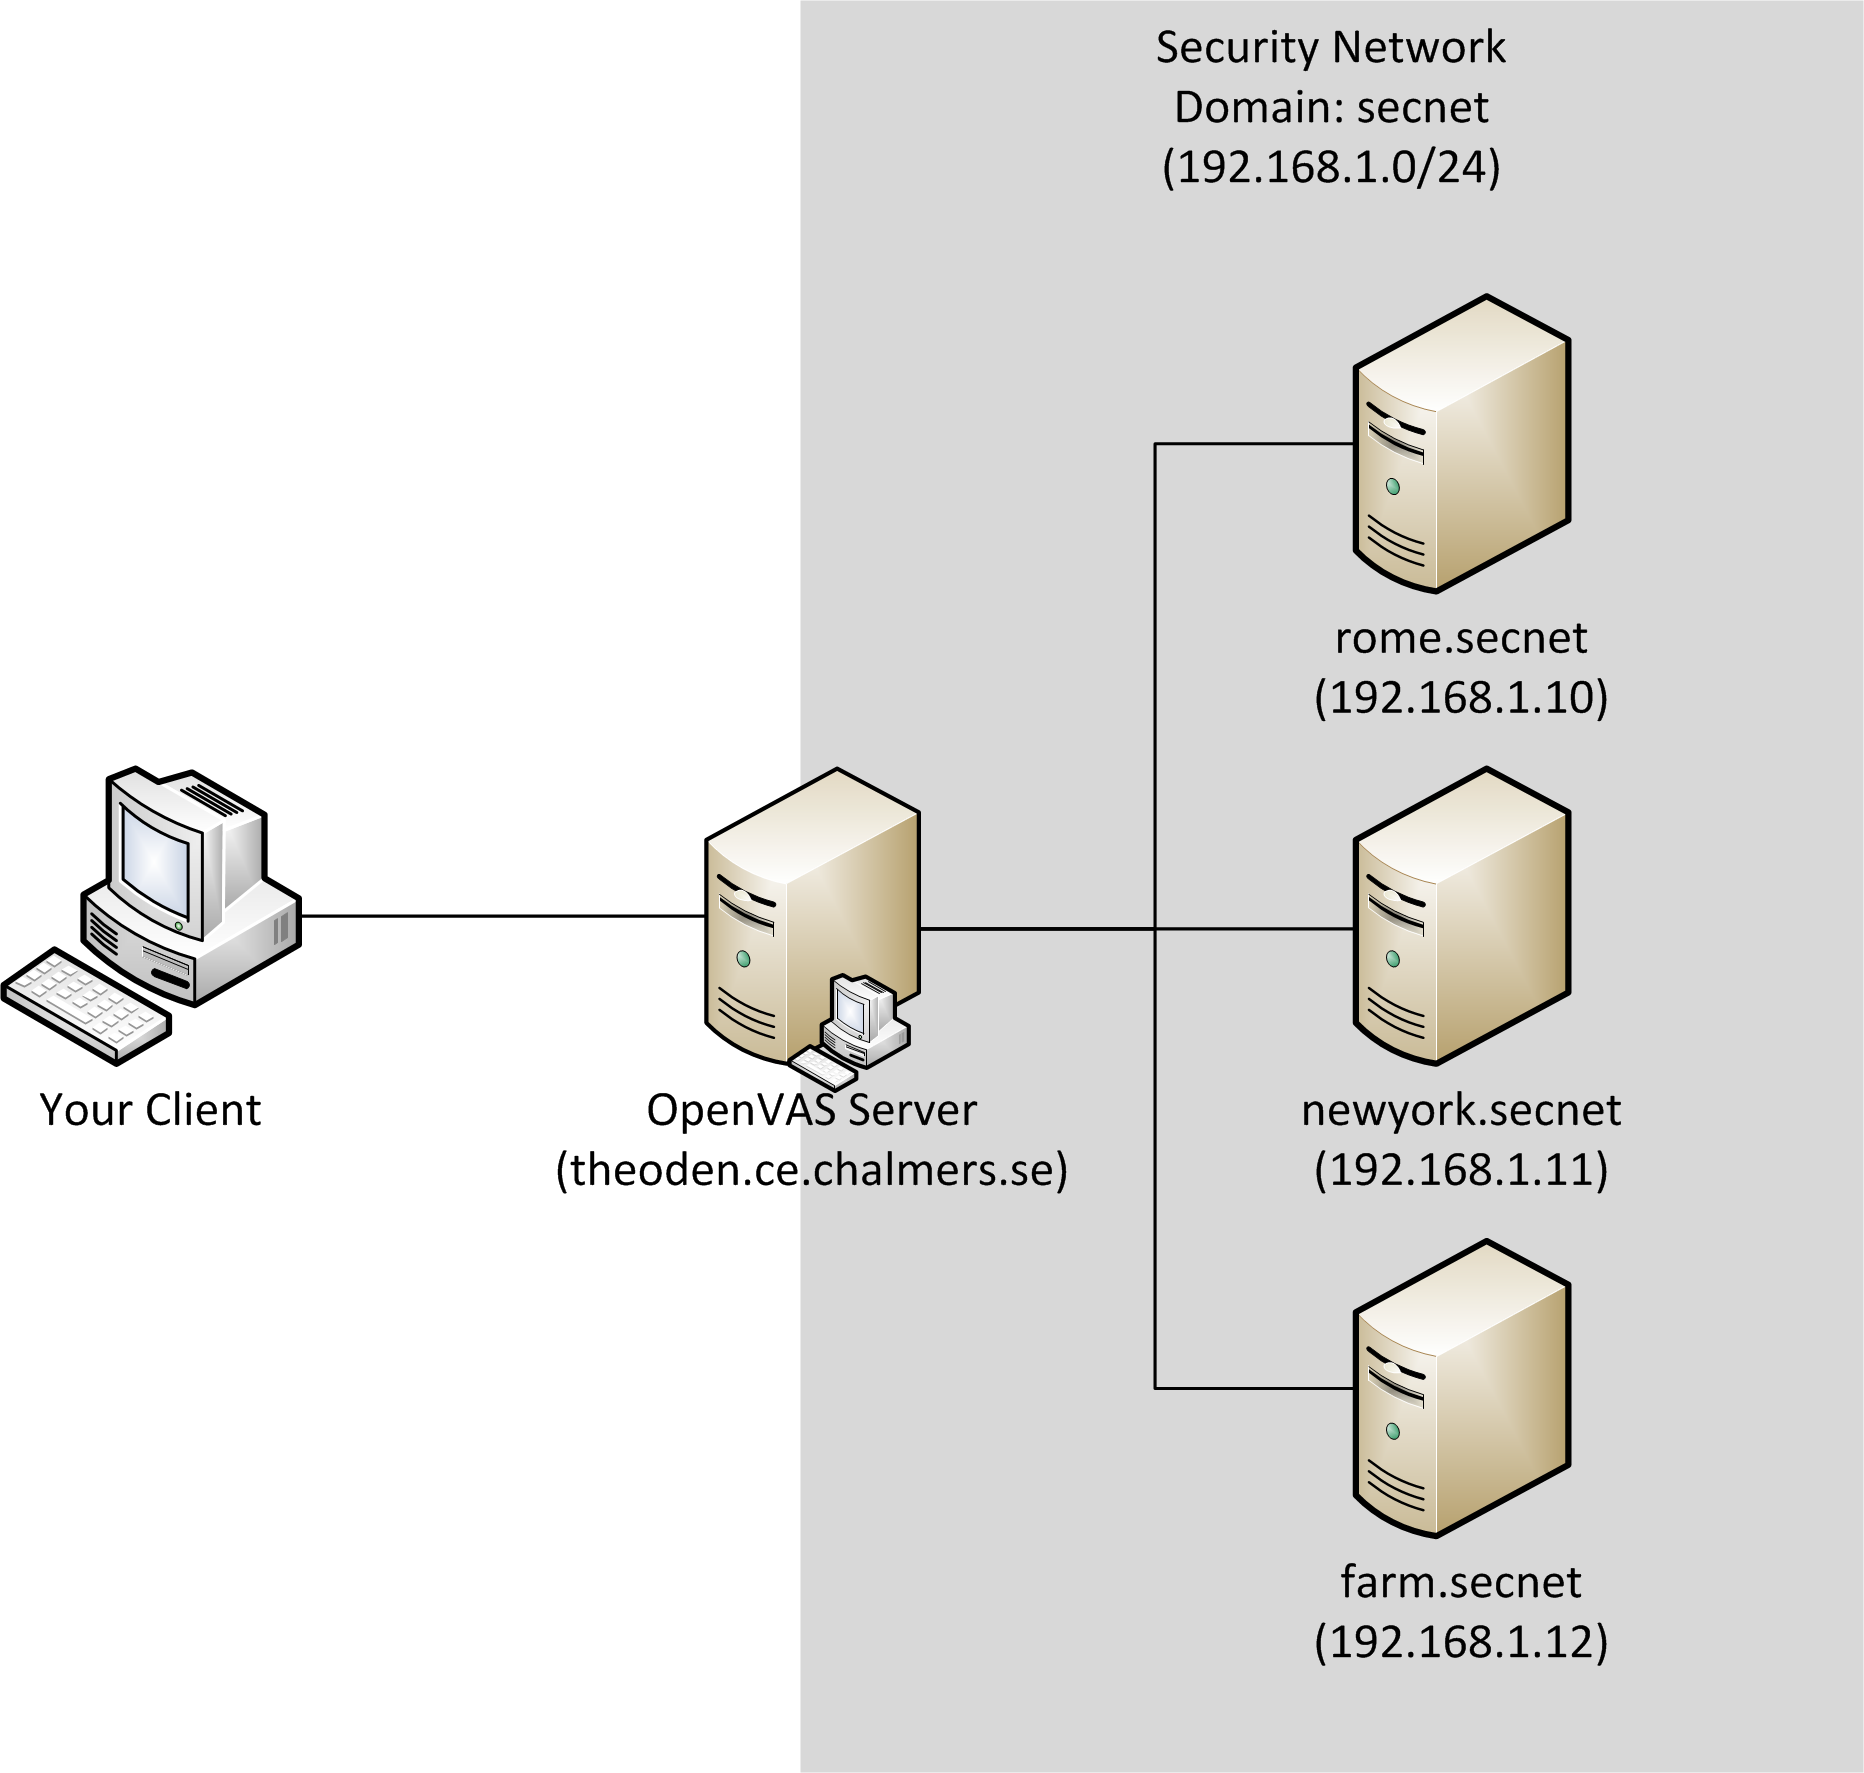
\includegraphics[scale=.4]{figures/setup.png}
  \caption{The laboratory network setup} \label{fig:setup}
\end{figure}



\subsection{Port Scanning}

\inlinetodo{text, figures, and tables if needed. Figure captions are below of figures, and Table caption should be above them.}


\subsection{Fingerprinting}

\inlinetodo{text, figures, and tables if needed}


\subsubsection{Service Fingerprinting}
\inlinetodo{text, figures, and tables if needed}

\subsubsection{Remote Host Fingerprinting}
\inlinetodo{text, figures, and tables if needed}


\subsection{Vulnerability Scanning}

\inlinetodo{text, figures, and tables if needed}
